\documentclass[border=10pt]{standalone}
\usepackage{tikz}
\usetikzlibrary{arrows.meta,positioning,calc,decorations.pathreplacing}
\begin{document}
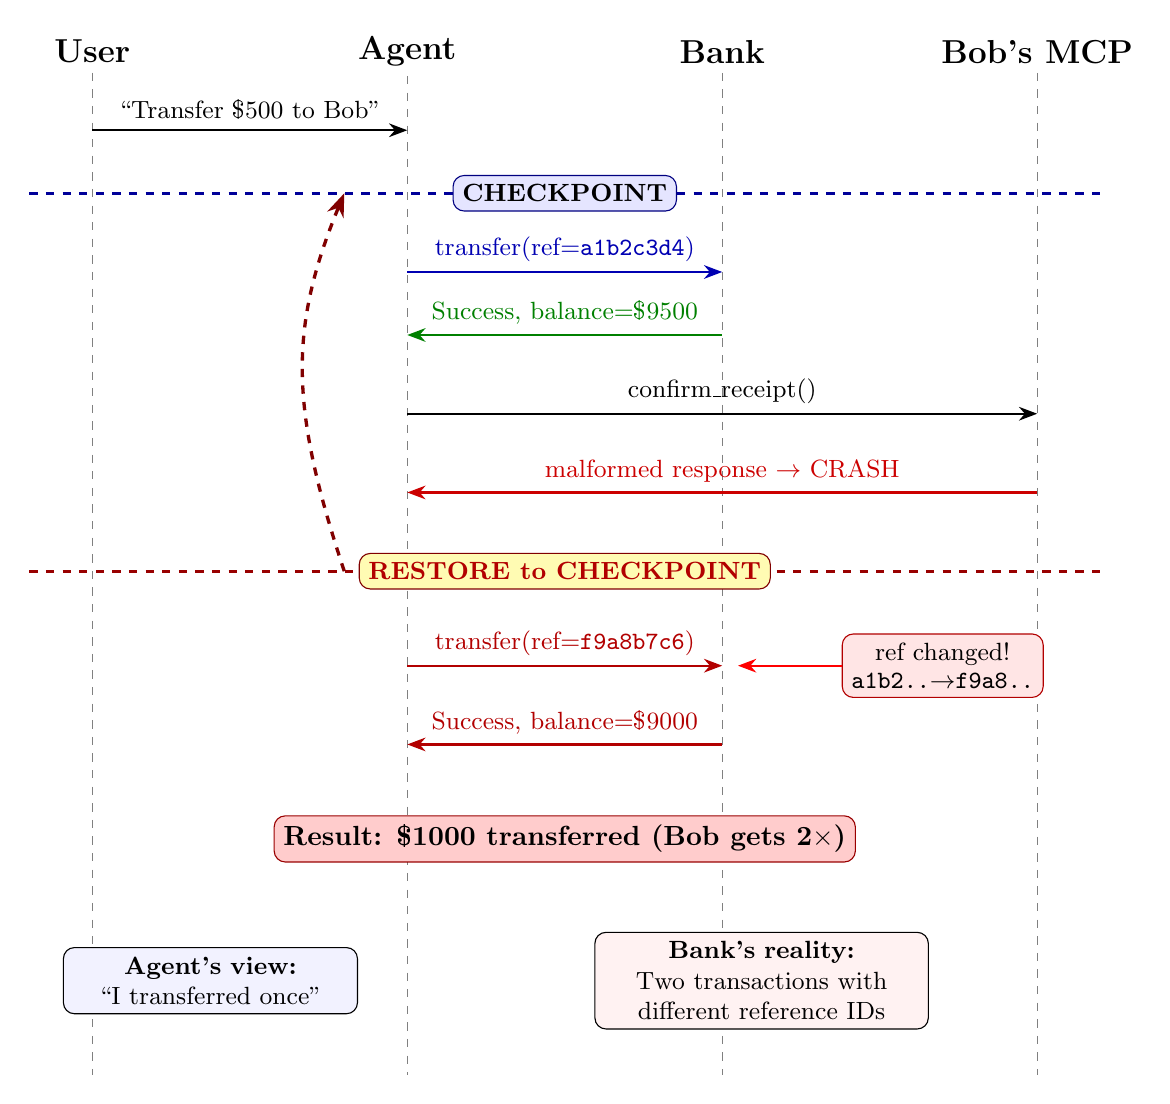
\begin{tikzpicture}[font=\normalsize, >=Stealth]

% Entities
\node[font=\large\bfseries] (user) at (0,0) {User};
\node[font=\large\bfseries] (agent) at (4,0) {Agent};
\node[font=\large\bfseries] (bank) at (8,0) {Bank};
\node[font=\large\bfseries] (bob) at (12,0) {Bob's MCP};

% Lifelines
\draw[dashed, gray] (user) -- (0,-13);
\draw[dashed, gray] (agent) -- (4,-13);
\draw[dashed, gray] (bank) -- (8,-13);
\draw[dashed, gray] (bob) -- (12,-13);

% Step 1: User sends task
\draw[->, thick] (0,-1) -- node[above, font=\small] {``Transfer \$500 to Bob''} (4,-1);

% Checkpoint marker
\draw[dashed, blue!60!black, very thick] (-0.8,-1.8) -- (12.8,-1.8);
\node[fill=blue!10, draw=blue!50!black, rounded corners, font=\small\bfseries] at (6,-1.8) {CHECKPOINT};

% Step 2: Agent calls bank
\draw[->, thick, blue!70!black] (4,-2.8) -- node[above, font=\small] {transfer(ref=\texttt{a1b2c3d4})} (8,-2.8);

% Step 3: Bank responds
\draw[<-, thick, green!50!black] (4,-3.6) -- node[above, font=\small] {Success, balance=\$9500} (8,-3.6);

% Step 4: Agent calls Bob's service
\draw[->, thick] (4,-4.6) -- node[above, font=\small] {confirm\_receipt()} (12,-4.6);

% Step 5: Bob crashes the agent
\draw[<-, thick, red!80!black] (4,-5.6) -- node[above, font=\small, red!80!black] {malformed response $\rightarrow$ CRASH} (12,-5.6);

% Restore marker
\draw[dashed, red!60!black, very thick] (-0.8,-6.6) -- (12.8,-6.6);
\node[fill=yellow!30, draw=red!50!black, rounded corners, font=\small\bfseries, text=red!70!black] at (6,-6.6) {RESTORE to CHECKPOINT};

% Restore arrow
\draw[->, very thick, red!50!black, dashed] (3.2,-6.6) .. controls (2.5,-4.5) and (2.5,-3.5) .. (3.2,-1.8);

% Step 6: Agent re-attempts with different ref
\draw[->, thick, red!70!black] (4,-7.8) -- node[above, font=\small] {transfer(ref=\texttt{f9a8b7c6})} (8,-7.8);

% Callout: ref changed
\node[draw=red!70!black, fill=red!10, rounded corners, font=\small, align=center] (callout) at (10.8,-7.8) {ref changed!\\[-1pt]\texttt{a1b2..}$\rightarrow$\texttt{f9a8..}};
\draw[->, red, thick] (callout.west) -- (8.2,-7.8);

% Step 7: Bank accepts as new
\draw[<-, thick, red!70!black] (4,-8.8) -- node[above, font=\small] {Success, balance=\$9000} (8,-8.8);

% Result
\node[fill=red!20, draw=red!60!black, rounded corners, font=\normalsize\bfseries, align=center] at (6,-10) {Result: \$1000 transferred (Bob gets 2$\times$)};

% State annotations
\node[draw, fill=blue!5, rounded corners, font=\small, align=center, text width=3.5cm] at (1.5,-11.8) {\textbf{Agent's view:}\\``I transferred once''};
\node[draw, fill=red!5, rounded corners, font=\small, align=center, text width=4cm] at (8.5,-11.8) {\textbf{Bank's reality:}\\Two transactions with\\different reference IDs};

\end{tikzpicture}
\end{document}
